\documentclass[crop,border=0pt]{standalone}

\usepackage{mathtools}
\usepackage{tikz}
\usetikzlibrary{positioning,scopes,arrows}

\begin{document}
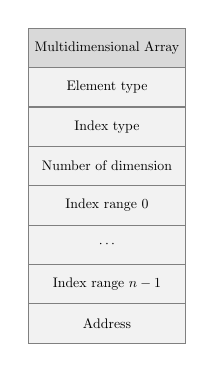
\begin{tikzpicture}[scale=0.5, every node/.style={scale=0.5,black}]
  {[xstep=4cm, ystep=1cm, gray, thin]

    \draw[fill=gray!10] (0, 0) grid (4, 7) rectangle (0, 0);
    \draw[fill=gray!30] (0, 7) grid (4, 8) rectangle (0, 7);

    \node at (2, 7.5) {Multidimensional Array};
    \node at (2, 6.5) {Element type};
    \node at (2, 5.5) {Index type};
    \node at (2, 4.5) {Number of dimension};
    \node at (2, 3.5) {Index range 0};
    \node at (2, 2.5) {\(\cdots\)};
    \node at (2, 1.5) {Index range \(n - 1\)};
    \node at (2, 0.5) {Address};
  }

\end{tikzpicture}
\end{document}
